\documentclass{IEEEtran}
\usepackage[utf8]{inputenc}
\usepackage{graphicx}
\usepackage{svg}
\usepackage{amsmath}
\usepackage{amsfonts}
\usepackage[hidelinks]{hyperref}
\usepackage[normalem]{ulem}
\usepackage{cite}
\usepackage[noabbrev]{cleveref} 
%
\usepackage{transparent}
\usepackage[caption=false, font=footnotesize]{subfig}
\usepackage{ulem}
\usepackage{multirow}
\usepackage{dcolumn}
\usepackage{lettrine}

\usepackage{siunitx}
\sisetup{load-configurations = abbreviations}
\usepackage{amssymb,latexsym}
\usepackage[american]{circuitikz}
\usepackage{gensymb}
\usepackage{verbatim}
\usepackage{booktabs}
\usepackage{csquotes}
% 
\usepackage{todonotes}
\usepackage{lipsum}

\def\sectionautorefname{Sec.}
\def\subsectionautorefname{Sec.}
\def\subsubsectionautorefname{Sec.}
\def\figureautorefname{Fig.}
\def\tableautorefname{Tab.}
\def\equationautorefname~#1\null{%
	(#1)}

\graphicspath {{./fig/}}

\newcommand{\figref}  [1] {\text{Fig}~\autoref{#1}}
\newcommand{\tabref}  [1] {\text{Tab.}~\autoref{#1}}
\newcommand{\subfigureautorefname}{\figureautorefname} 
\newcommand{\grad}{\nabla}
\newcommand{\divergence}{\grad \cdot}
\newcommand{\curl}{\grad \times}
\newcommand{\laplacian}{\grad^2}
\newcommand{\iu}{j}

\newcommand{\chargeDensity}{\rho}
\newcommand{\conductivity}{\sigma}
\newcommand{\permittivity}{\varepsilon}
\newcommand{\effectivePermittivity}{\permittivity_e}
\newcommand{\permeability}{\mu}
\newcommand{\complexPermeability}{\mbox{\boldmath $\permeability$}}
\newcommand{\magneticSusceptibility}{\chi}
\newcommand{\skinDepth}{\delta}
\newcommand{\wavelength}{\lambda}


\newcommand{\SWR}{\text{SWR}}
\newcommand{\SRF}{\text{SRF}}
\newcommand{\complexInductance}{\mbox{\boldmath $L$}}

\newcommand{\impedance}{Z}
\newcommand{\impedanceIn}{\impedance_{\text{in}}}
\renewcommand{\Re}{\mathbb{R}e}
\renewcommand{\Im}{\mathbb{I}m}



\newcommand{\complexImpedance}{\mbox{\boldmath $Z$}}
\newcommand{\complexAdmittance}{\mbox{\boldmath $Y$}}
\newcommand{\complexResidue}{\mbox{\boldmath $r$}}
\newcommand{\complexPole}{\mbox{\boldmath $p$}}
\newcommand{\complexCte}{\mbox{\boldmath $d$}}
\newcommand{\complexProp}{\mbox{\boldmath $e$}}

\newcommand{\SEMBA}{\textit{SEMBA-FDTD }}

\newcommand{\citetemp}[1]{(#1)}
\newcounter{mytempeqncnt}


\author{
	Author 1, Author 2, Author 3$^{*}$, \newline Author 4, Author 5, and Author 6, {\em IEEE Senior Member}
	\thanks{The 1st, 2nd, 3rd, 4th, and 7th authors are with the XXXX, in University of Granada, Spain. 
		5th author is with YYYY company.
		6th author is with ZZZZ institution. 
		* Corresponding author e-mail: \texttt{xxx@yyy.zzz}.}
	\thanks{The work described in this paper and the research leading to these results were supported by the 
		XXXX grants. 
	}
}
\date{\today}
\title{Paper Title: This is a template for an IEEE submission}

\begin{document}
	\maketitle
	
	\begin{abstract}
		The abstract
	\end{abstract}
	
	\begin{IEEEkeywords}
		keywords must be lowercased,
		common mode chokes,
		ferrite,
		complex permeability,
		multi conductor transmission lines
	\end{IEEEkeywords}
	
	\section{Introduction}\label{sec:introduction}
\IEEEPARstart{C}{ommon} mode (CM) ferrite chokes are essential components used for electromagnetic compatibility (EMC) purposes 
\todo[inline]{ToDo notes can be used temoprarily to mark pending work that must be done before submitting.}
\todo[inline]{State the purpose of this work}
\todo[inline]{Reference to current state-of-the-art}
\todo[inline]{Explain the organization of the paper.}

Units can be written in SI as \SI{+20}{dB/dec}.

A citation example \cite{Lee2021,Barba2020,Kacki2023}. 
This references must be located in the \texttt{bibliography/references.bib} file, using \texttt{bibtex} format.
	\section{Experimental and simulation results} \label{sec:experimental-and-simulation-results}
Something something $L=\SI{6}{mm}$ and $W=\SI{3}{mm}$
\begin{figure*}[ht]
	\centering
	\subfloat[Caption of first figure]{
		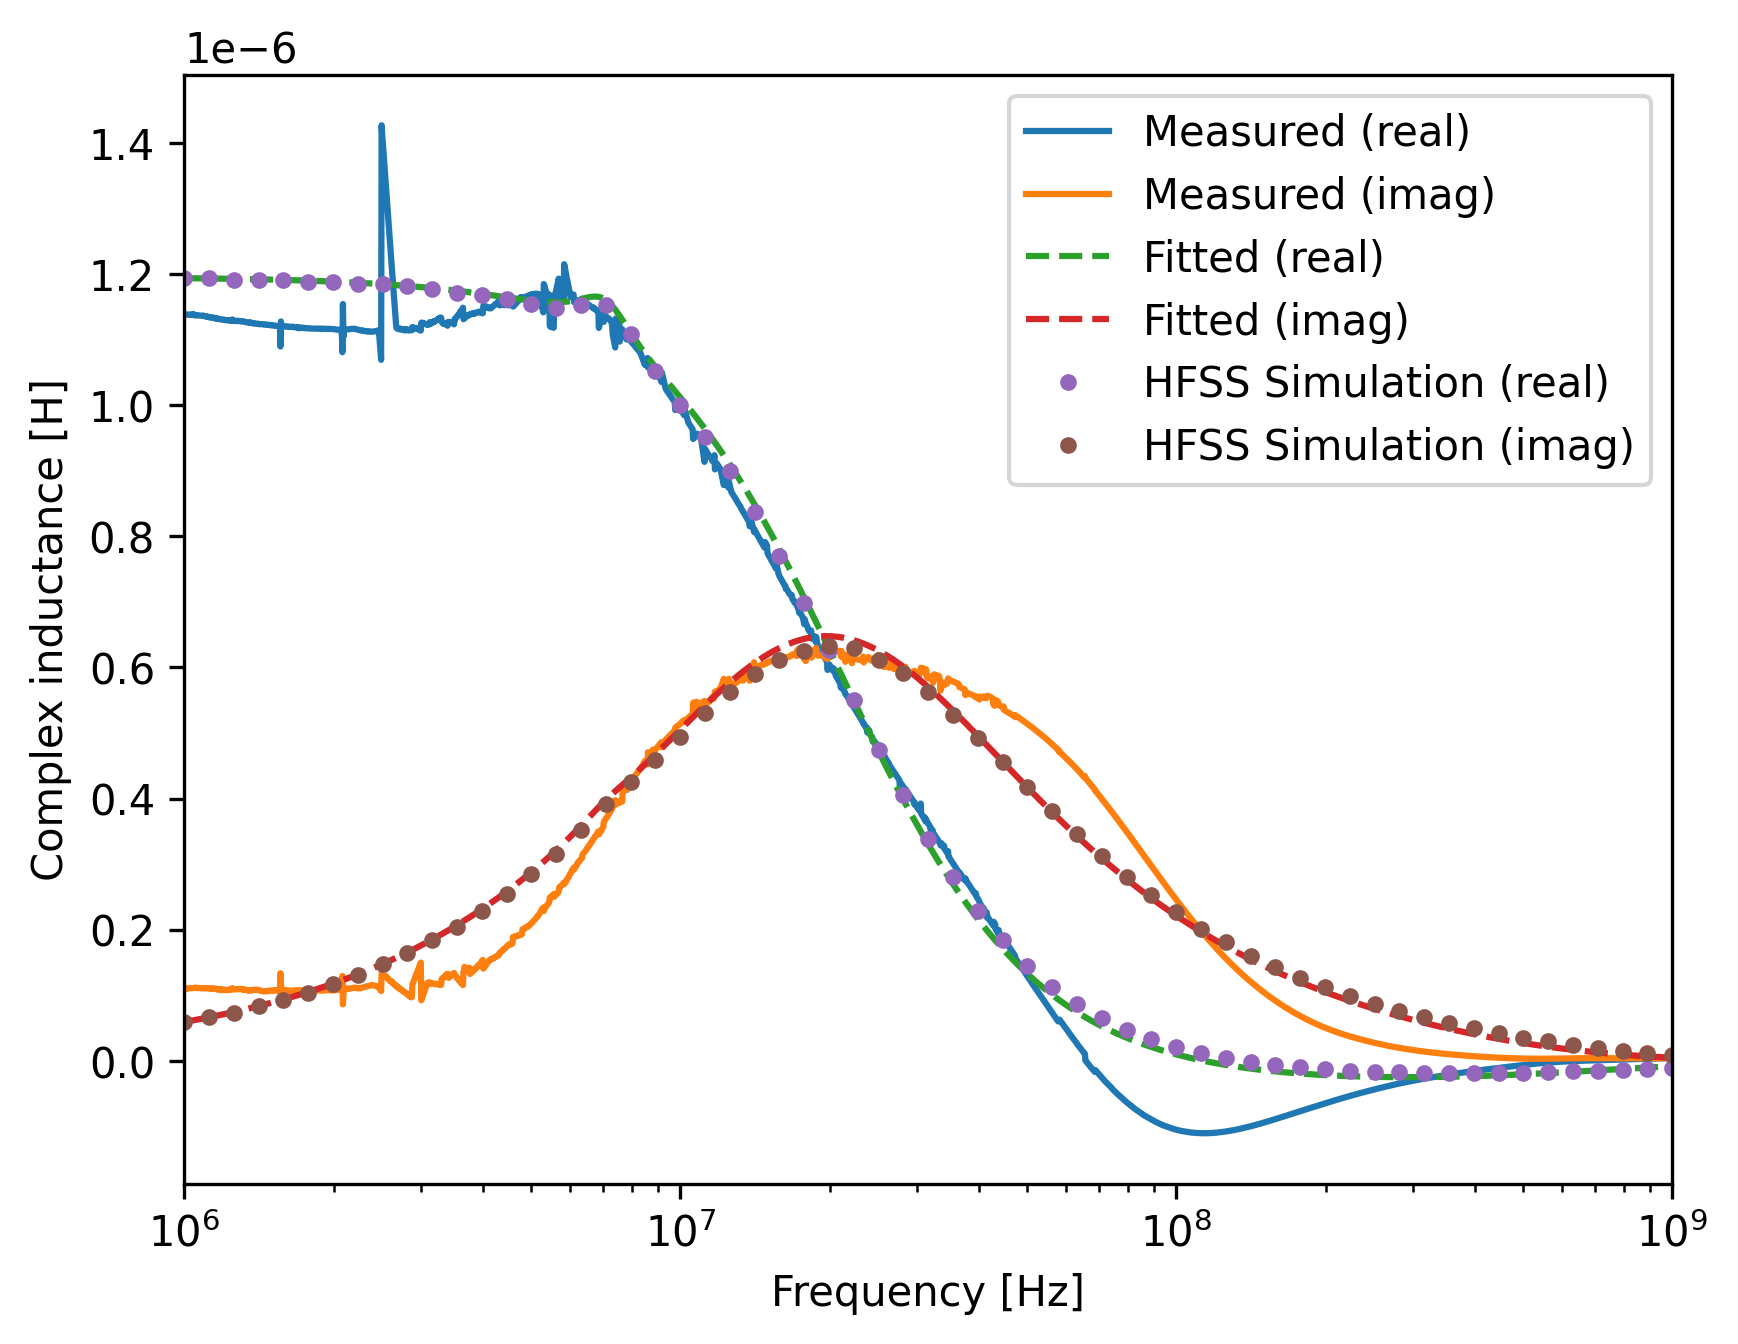
\includegraphics[width=0.45\textwidth]{inductance-measurements-and-fitting}
	}
	\subfloat[Caption of second figure]{
		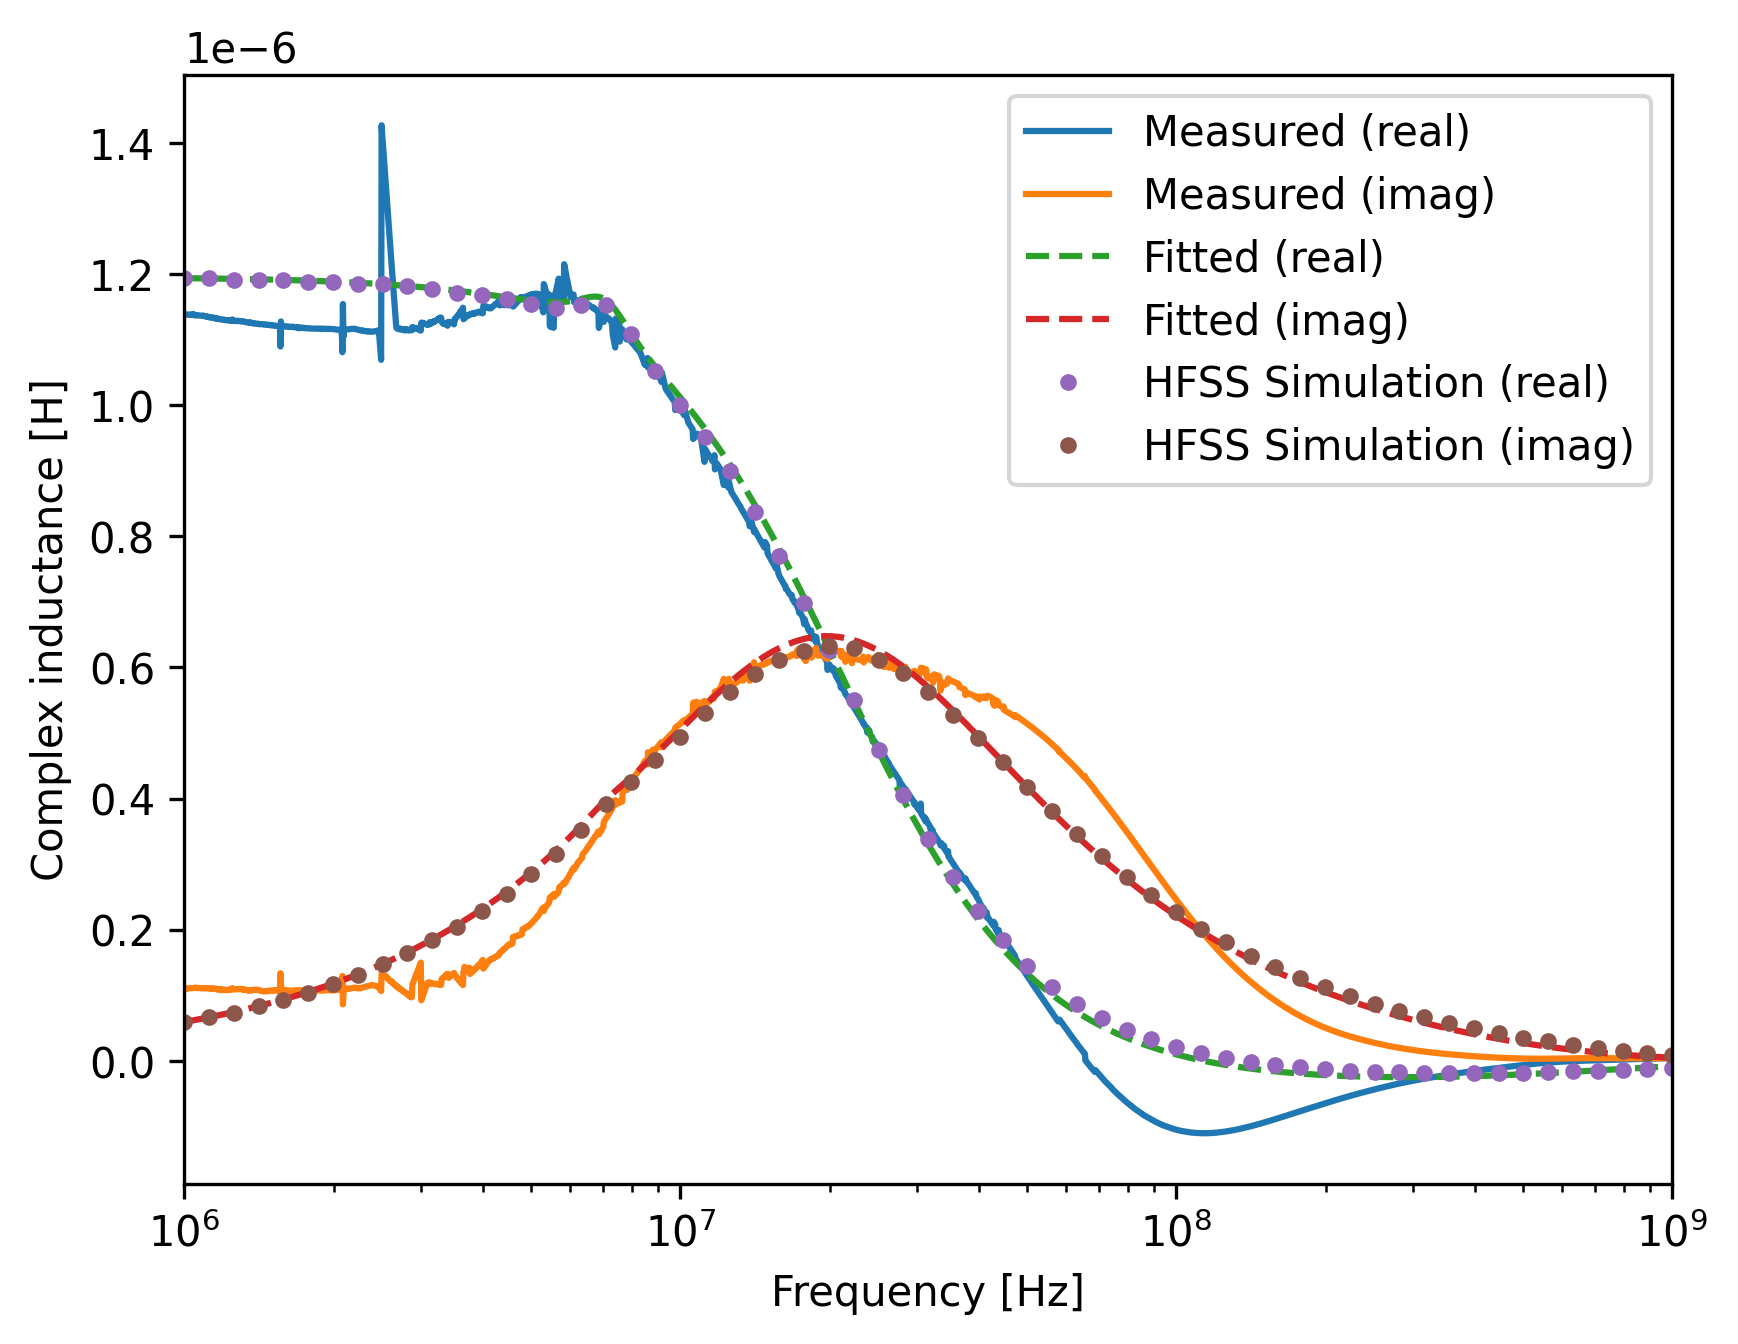
\includegraphics[width=0.45\textwidth]{inductance-measurements-and-fitting}
	}
	\caption{Example of figure}
	\label{fig:inductance-measurement}
\end{figure*}

\subsection{Experimental setup} \label{sec:experimental-setup}
In Ohm's law,
\begin{equation}
	V = R I \label{eq:ohms-law}
\end{equation}

Text can include references to figures \autoref{fig:inductance-measurement}, to sections \autoref{sec:introduction} and to equations \autoref{eq:ohms-law}.

\subsection{Simulations}
More complex formulas can be placed using \texttt{align} environment
\begin{align}
	\complexImpedance & = \iu\omega \complexInductance_{fit} \\
	& = \iu\omega \complexPermeability_{fit} \ln\left(\frac{r_e}{r_i}\right)\frac{h}{2\pi} \\
	& = \iu\omega (\mu_{fit}^{\prime}-\iu\mu_{fit}^{\prime\prime}) \ln\left(\frac{r_e}{r_i}\right)\frac{h}{2\pi}
\end{align}
In figure \autoref{fig:circuit-example} we show an example of a circuit written in latex.
Missing figures that are not available while writting the paper can be placed temoprarily \autoref{fig:circuit-example}

\begin{figure}[ht]
	\begin{circuitikz}[scale=1]
		\draw
		(0,2) to[vsource, l=\SI{48}{\volt}]
		(0,0) to[short, -*]
		(6,0) to[short, -o]
		(8,0)
		(0,2) to[R, l=$R_x$, -*]
		(2,2) to[short]
		(2,1) to[R, l=\SI{4}{\ohm}]
		(4,1) to[short,-*]
		(4,2)
		(2,2) to[short]
		(2,3) to[isource,l=\SI{3}{\ampere}, invert]
		(4,3) to[short,-*]
		(4,2) to[short,-*]
		(6,2) to[short, i=$i$, -o]
		(8,2) to[open, v=$v$]
		(8,0)
		(6,2) to[R,l=\SI{12}{\ohm}]
		(6,0);
	\end{circuitikz}
	\caption{This is an example of a circuit}
	\label{fig:circuit-example}
\end{figure}

\begin{figure}[ht]
	\centering
	\missingfigure{Experimental setup}
	\caption{Example of missing figure.}
	\label{fig:missing-figure}
\end{figure}
	\section{Conclusions}\label{sec:conclusions}

\todo[inline]{Conclusions}
	
	\section{Acknowledgements}	
	The authors want to thank these people for this and that company for that.

	\bibliographystyle{IEEEtran}
	\bibliography{bibliography/references.bib}
	
\end{document}
